\justifying
We also instantiate the NC abstraction in interactive desktop environments with \ncguiworld{}.
In this setting, fine-grained action control is essential: GUI interaction requires precise cursor tracking, timely click feedback, and robustness to rapidly changing interface states.
We model each interaction as a synchronized sequence of RGB frames $x_t$ and input events $u_t$ (mouse and keyboard).
The latent video state maintains interface context across frames, while temporally aligned action inputs provide control signals designed to preserve pixel-level correspondence between user actions and visual changes.


\subsubsection{Data pipeline}
\label{section:impl-guiworld-data-pipeline}
\begin{wraptable}{r}{0.48\linewidth}
  \vspace{-1.7em}
  \captionsetup{type=table,width=\linewidth}
  \centering
  \small
  \rowcolors{2}{metablue!8}{white}
  \caption{Cursor/action statistics.}
  \label{tab:gui-stats}
  \setlength{\tabcolsep}{7pt}
  \begin{tabularx}{\linewidth}{l >{\centering\arraybackslash}X >{\centering\arraybackslash}X}
    \toprule
    \rowcolor{metablue!16}\textbf{Split} & \textbf{Avg. cursor speed (px/frame)} & \textbf{Actions / sec} \\
    Random Slow & 1.51 & 1.58 \\
    Random Fast & 195.15 & 4.18 \\
    CUA (supervised) & 3.79 & 0.10 \\
    \bottomrule
  \end{tabularx}
  \vspace{-0.8em}
\end{wraptable}

% We collect GUI data at 15~FPS with synchronized cursor and keyboard logs. 
The dataset includes two styles of random interaction: ``Random Slow'' and ``Random Fast'', plus a smaller set of supervised trajectories collected by Claude CUA~\citep{claudeComputerTool}.
Random Slow (approximately 1{,}000 hours) contains longer pauses, idle gaps, and deliberate cursor movements, which can expose cursor drift after extended inactivity.
Random Fast (approximately 400 hours) features denser cursor motion and typing bursts, stressing acceleration dynamics and hover timing.
%
The supervised trajectories are approximately 110 hours. 
These goal-directed traces provide higher-signal action--response pairs without overwhelming the exploration data.
Table~\ref{tab:gui-stats} summarizes cursor and action statistics across splits; in the collected CUA trajectories, action density is lower due to latency introduced by Claude’s tool API between successive steps.


All GUI data is collected inside an Ubuntu~22.04 container running XFCE4 (Arc-Dark theme, Papirus icons) on a fixed 1024$\times$768 virtual display at 15~FPS.
We render the display with Xvfb and interact through a VNC/noVNC stack.
The desktop pins a small open-source app set to launchers.
It includes Firefox ESR, GIMP, VLC, VS~Code, Calculator, Terminal, the file manager, and the Mahjongg game, matching the environment shown in our recordings.
Screen capture uses \texttt{mss} and \texttt{ffmpeg} with cursor overlays, and actions are replayed and logged via \texttt{xdotool}.
%
We keep the recorded discontinuities and interface latency intact rather than smoothing them.
In dataset packaging, we store both raw-action and meta-action views for modeling.
This lets us train either the raw-action or meta-action encoder under the same loss stack\footnote{Conversion details and alignment quality appear in Appendix~\ref{appendix:gui-actions}.}.







\subsubsection{Model architecture}


The GUIWorld architecture builds on the Wan2.1~\citep{wan2025wan} by incorporating explicit action-conditioning modules.
The central challenge is to align time-stamped user actions with generated frames and inject this information at the appropriate depth within the transformer.


Action features are encoded on-the-fly from frame-aligned mouse and keyboard signals (Section~\ref{section:impl-guiworld-data-pipeline}).
We aggregate them into latent-aligned embeddings that summarize recent action history at each diffusion step.
%
We evaluate two action encoders.
The \emph{raw-action encoder} (v1) preserves fine-grained mouse/keyboard event streams.
The \emph{meta-action encoder} (v2) abstracts interactions into coarse API-style categories (clicks, drags, scrolls, typing, shortcuts).
Both encoders use the same temporal alignment and are evaluated as separate ablations.
In our experiments, their differences in rendering fidelity and control behavior are modest\footnote{Appendix Table~\ref{tab:action-encoder-comparison} summarizes the representational differences.}.


We inject action embeddings into the diffusion backbone in four ways (Figure~\ref{fig:action-injection}).
We study \texttt{external}, \texttt{contextual}, \texttt{residual}, and \texttt{internal} conditioning.
For the injection-scheme ablation, all four modes share the same meta-action encoder and temporal alignment.
They differ only in where the latent action features interact with the video latents and transformer blocks.
We compare raw-action vs.\ meta-action encoders separately in Table~\ref{tab:gui-encoding-ablation}.



\noindent\textbf{External conditioning.}
In the \texttt{external} mode, action information modulates the latent video sequence before the diffusion transformer.
Action features are applied as a pre-conditioning step at the model input, without introducing explicit action tokens or cross-attention inside the diffusion backbone.
As a result, action information enters only through the modified input latents; the diffusion backbone never attends directly to action tokens, so any action signal must be carried implicitly in $z'_{1:T}$.

Formally, given VAE latents $z_{1:T}$ and temporally aligned action features $u_{1:T}$, an external action module applies a small stack of temporal self-attention and action cross-attention layers.
This produces a residual update $\Delta z_{1:T}(u_{1:T})$.
The modified latents are
\[
  z'_{1:T} = z_{1:T} + \Delta z_{1:T}(u_{1:T}),
\]
and the diffusion transformer operates solely on $z'_{1:T}$.
The diffusion backbone remains unchanged, and action features are not exposed as explicit tokens within the transformer.



\begin{figure}[t]
  \centering
  \DeclareRobustCommand{\modeExt}{\tikz[baseline=-0.2em]{\node[fill=red!70, circle, inner sep=1.6pt, text=white, font=\scriptsize]{1};}}
  \DeclareRobustCommand{\modeCtx}{\tikz[baseline=-0.2em]{\node[fill=blue!70, circle, inner sep=1.6pt, text=white, font=\scriptsize]{2};}}
  \DeclareRobustCommand{\modeRes}{\tikz[baseline=-0.2em]{\node[fill=orange!80, circle, inner sep=1.6pt, text=white, font=\scriptsize]{3};}}
  \DeclareRobustCommand{\modeInt}{\tikz[baseline=-0.2em]{\node[fill=teal!70, circle, inner sep=1.6pt, text=white, font=\scriptsize]{4};}}
  
\includegraphics[width=\linewidth]{assets/action_injection4.pdf}
  \vspace{0.2em}
  \small
  \setlength{\tabcolsep}{4pt}
  \renewcommand{\arraystretch}{1.05}
  \begin{tabularx}{\linewidth}{@{}l >{\raggedright\arraybackslash}p{0.30\linewidth} X@{}}
    \toprule
    \textbf{Mode} & \textbf{Injection point} & \textbf{Notes} \\
    \modeExt\ \texttt{external} & Conditioned VAE input & Actions are injected as an external conditioning stream that modulates the backbone without sharing the main token sequence. \\
    \modeCtx\ \texttt{contextual} & Concat frames, actions & Video and action tokens share one sequence with a lag-aware temporal attention mask, enabling mid-level fusion. \\
    \modeRes\ \texttt{residual} & Hidden state with action delta & Actions are added through residual-style modulation branches, acting as a strong but more indirect baseline. \\
    \modeInt\ \texttt{internal} & After cross-attn, before FFN & Actions enter through dedicated cross-attention inside the transformer blocks, fusing near the backbone core. \\
    \bottomrule
  \end{tabularx}
  \vspace{0.1em}
  \captionsetup{justification=raggedright,singlelinecheck=false}
\caption{\textbf{Four modes for injecting GUI actions into the diffusion transformer.}
\modeExt{} modulates VAE latents before the transformer;
\modeCtx{} adds action tokens alongside visual tokens;
\modeRes{} applies block-wise residual updates; and
\modeInt{} inserts an action cross-attention module inside transformer blocks.}

  \label{fig:action-injection}
\end{figure}

\noindent\textbf{Contextual conditioning.}
In the \texttt{contextual} mode, actions are represented as additional tokens and integrated directly into the transformer’s self-attention.
Similar token-based action representations have been explored in prior world models, including Gato~\citep{reed2022generalist} and World and Human Action Models~\citep{kanervisto2025world}.

The meta-action encoder produces latent-aligned action tokens $A \in \mathbb{R}^{L_a \times D}$.
We concatenate them with visual tokens $V \in \mathbb{R}^{L_v \times D}$ to form a joint sequence $[V; A]$.
Each transformer block applies self-attention over this combined sequence using a structured temporal mask (Appendix Figure~\ref{fig:contextual-mask}).
The mask enforces causal alignment: each frame token attends only to actions within a short past window, and each action token attends only to frames after a fixed temporal lag.
Through this masked joint attention, \texttt{contextual} conditioning fuses action and visual information within the transformer blocks.


\noindent\textbf{Residual conditioning.}
In the \texttt{residual} mode, the transformer block structure remains unchanged.
A lightweight action module attaches to a subset of layers as an external residual branch.
This follows the \texttt{residual} conditioning paradigm introduced by ControlNet~\citep{zhang2023adding}, while remaining modular and additive to the base diffusion backbone.

At each selected layer $l$, the transformer applies its standard sequence of self-attention, text or reference cross-attention, and feed-forward operations to produce hidden states $h^{(l)}$.
A separate action module then takes $h^{(l)}$ together with a local temporal window of latent action features and mouse trajectories.
It outputs a residual update $\Delta h^{(l)}(a,\text{mouse})$.
The updated hidden states are given by
\[
  \tilde{h}^{(l)} = h^{(l)} + \Delta h^{(l)}(a,\text{mouse}),
\]
which are passed to the subsequent transformer block.
In this formulation, \texttt{residual} conditioning injects action information through block-external residual branches.
It does not modify the internal computations of the transformer blocks themselves.


\noindent\textbf{Internal conditioning.}
In the \texttt{internal} mode, action conditioning is incorporated directly within the transformer blocks.
Related multi-stream world models have explored similar designs, including Matrix-Game-2~\citep{he2025matrix}.
Each selected block augments the standard attention stack with an additional action cross-attention sub-layer.
Specifically, the block applies self-attention, followed by cross-attention over text and reference features, and then a dedicated action cross-attention layer.
Keys and values are derived from latent action features (and, optionally, mouse inputs).

Given block input $h$, text or reference context $c$, and action latents $a$, the internal block computes
\[
  h' = \mathrm{FFN}\Big(
    h + \mathrm{CA}_{\text{text}}\big(\mathrm{SA}(h), c\big)
      + \mathrm{CA}_{\text{action}}(h, a)
  \Big),
\]
where $\mathrm{SA}$ denotes self-attention and $\mathrm{CA}_{\text{text}}$ and $\mathrm{CA}_{\text{action}}$ denote the text and action cross-attention modules applied in sequence.
As illustrated in Figure~\ref{fig:action-injection}, action features are injected directly into the block’s cross-attention stage.

In contrast to \texttt{residual} conditioning, \texttt{internal} conditioning integrates action information through a block-internal attention mechanism rather than an external residual branch.
This design mirrors the multi-stream injection strategy used in Matrix-Game-2~\citep{he2025matrix} and yields the best SSIM/FVD trade-off for fine-grained GUI interaction in our ablations.
In this setting, precise temporal alignment and spatial locality are critical.
Each conditioning mode (\texttt{external}, \texttt{contextual}, \texttt{residual}, and \texttt{internal}) is trained as a separate ablation, and no combinations are used.


\subsubsection{Implementation Details}
We train one model per injection mode (\texttt{external}, \texttt{contextual}, \texttt{residual}, \texttt{internal}), keeping the backbone and all non-action components fixed.
Each run lasts about 64k steps.
We tune only the action encoder and learning-rate schedule.
Training optimizes the diffusion loss together with a small temporal contrastive loss that aligns frame features with action and mouse embeddings (Appendix~\ref{appendix:gui-actions}).
Runs use 64 GPUs for about 15 days, totaling about 23k GPU-hours per full pass.

Preprocessing is implemented in the data loader in two stages.
First, we normalize each recording to a fixed resolution and frame rate.
This produces tensors for RGB video, per-frame cursor coordinates, and mouse/keyboard event traces (in both raw-action and meta-action views).
Second, we render an SVG cursor at each logged position to produce per-frame masks and cursor-only reference frames.
The first reference frame contains the full desktop with a unit mask.
Later references paste only the cursor over a neutral background, with a mask restricted to arrow pixels.
After VAE encoding, these references become latent slots that pin down the static GUI layout at $t{=}0$.
For $t{>}0$, they supervise only a small patch around the cursor and leave the rest of the frame unconstrained.
We drop clips without valid cursor or action traces to keep~supervision~consistent.

\subsubsection{Evaluation setup}
Our ablations target three capabilities: global fidelity, post-action responsiveness, and cursor-control precision.
We use the \FVD/\LPIPS/\SSIM~suite as the core metrics.
We also add action-driven metrics that focus on post-interaction frames after clicks, scrolls, and key/type events.
For example, we compute \SSIM/\LPIPS~averaged over the $k$ frames after each logged action, and action-driven \FVD~on post-action clips.
Ablations vary conditioning design and action encoding to measure how these choices affect perceptual quality and responsiveness when rolled out against ground-truth interfaces\footnote{Full metric definitions and implementation details are provided in Appendix~\ref{appendix:gui-metrics}.}.


\exptitle[\guiworldLogo]{7}{Data quality dominates performance}



Interactive GUI modeling shows that data quality matters more than dataset size for action-driven performance.
We compare slow exploration, fast interaction, and supervised trajectories under \texttt{contextual} conditioning.
This isolates which behaviors best support neural computer training.




\begin{wraptable}{r}{0.48\linewidth}
  \vspace{-0.1em}
  \captionsetup{type=table,width=\linewidth}
  \centering
  \small
  \rowcolors{2}{metablue!8}{white}
  \caption{Overall performance across data sources.}
  \label{tab:gui-data-quality}
  \setlength{\tabcolsep}{7pt}
  \begin{tabularx}{\linewidth}{l >{\centering\arraybackslash}X >{\centering\arraybackslash}X >{\centering\arraybackslash}X}
    \toprule
    \rowcolor{metablue!16}\textbf{Split} & \textbf{FVD$_\text{all}$} & \textbf{SSIM$_\text{all}$} & \textbf{LPIPS$_\text{all}$} \\
    Untrained baseline & 149.61 & 0.496 & 0.605 \\
    Random Fast (train) & 48.17 & 0.695 & 0.483 \\
    Random Slow (train) & 20.37 & 0.830 & 0.237 \\
    Claude CUA (train) & 14.72 & 0.885 & 0.144 \\
    \bottomrule
  \end{tabularx}
  \vspace{-1.8em}
\end{wraptable}

Despite approximately 1{,}400 hours of random exploration across the slow and fast settings, these datasets are noisy.
They are comparatively sample-inefficient for learning stable action--response mappings.
They substantially improve global perceptual metrics over a baseline (Table~\ref{tab:gui-data-quality}).
However, high-frequency cursor jitter and irregular, non-goal-directed action bursts make consistent control difficult under dense, stochastic input streams.

In contrast, the substantially smaller high-quality dataset (110 hours from Claude CUA) yields markedly stronger performance across all metrics.
Goal-directed trajectories provide clearer action semantics and more predictable state transitions.
This enables robust action conditioning even with limited data volume.
These results indicate that neural computer development should prioritize curated, purposeful interactions over large-scale passive data collection.



\exptitle[\guiworldLogo]{8}{Precise cursor control requires explicit visual supervision}

\begin{figure}[h]
  \centering
  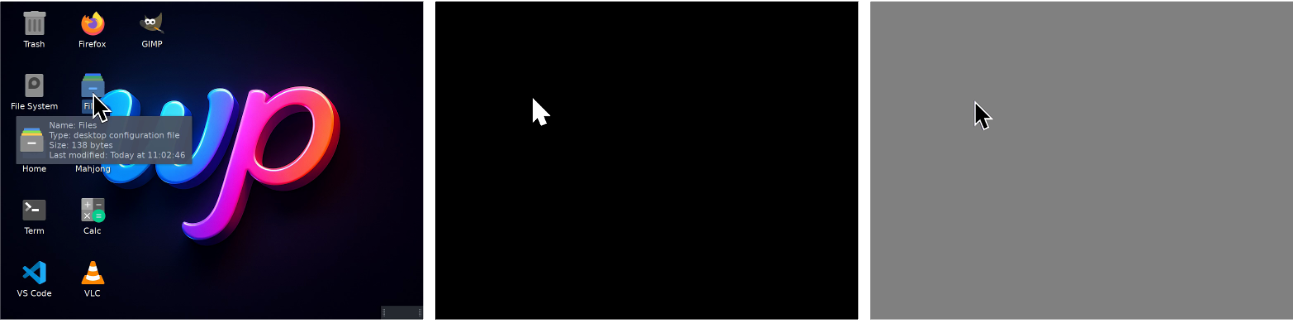
\includegraphics[width=\linewidth]{assets/ref2.png}
\caption{\textbf{Cursor references in GUIWorld.}
\textbf{Left:} original desktop frames.
\textbf{Middle:} binary cursor masks.
\textbf{Right:} cursor-only reference frames rendered over a neutral background.}
  \label{fig:cursor-ref}
\end{figure}

\begin{wraptable}{r}{0.48\linewidth}
  \vspace{-1.0em}
  \captionsetup{type=table,width=\linewidth}
  \centering
  \small
  \rowcolors{2}{metablue!8}{white}
  \caption{Cursor conditioning losses versus accuracy.}
  \label{tab:cursor-loss}
  \setlength{\tabcolsep}{7pt}
  \begin{tabularx}{\linewidth}{l >{\centering\arraybackslash}X}
    \toprule
    \rowcolor{metablue!16}\textbf{Loss variant} & \textbf{Cursor accuracy} \\
    Position $(x,y)$ only & 8.7\% \\
    Position $(x,y)$ + Fourier & 13.5\% \\
    Position $(x,y)$ + SVG mask/ref & \textbf{98.7\%} \\
    \bottomrule
  \end{tabularx}
  \vspace{-0.8em}
\end{wraptable}

We examine whether the NC internalizes cursor dynamics.
A natural baseline is to condition on normalized cursor-coordinate sequences $\texttt{mouse\_trajectories}\subset[0,1]^{T\times 2}$ (details in Appendix~\ref{appendix:mouse-traj-normalization}). 
%
To strengthen this signal, we further encode the normalized trajectories using a Fourier mouse encoder.
We map coordinates to $[-1,1]^2$ and project them through a fixed Gaussian matrix to obtain random Fourier features.
A small MLP produces per-frame embeddings, which we aggregate into lag-aware windows aligned with the VAE stride.
The resulting latent action sequence conditions the action modules and participates in the temporal contrastive loss.

However, Table~\ref{tab:cursor-loss} shows that coordinate-based supervision remains insufficient for precise interaction.
Position-only supervision achieves 8.7\% accuracy, and even enhanced position features reach only 13.5\%.
This suggests that richer coordinate encodings alone do not resolve cursor drift and jitter.

Motivated by the importance of precise cursor placement, we introduce explicit visual cursor supervision.
We render an SVG cursor at each $(x_t,y_t)$ to produce per-frame cursor masks $m_t$ and cursor-only foregrounds $f_t$ (right panel of Figure~\ref{fig:cursor-ref}).
Following Figure~\ref{fig:cursor-ref}, we construct a reference stream.
The first frame contains the full desktop image, while subsequent frames contain only the cursor foreground over a neutral background, masked to the cursor region.
We encode both the video and reference streams with the shared VAE, yielding video latents $z_{1:T}$, reference latents $z^{\text{ref}}_{1:T}$, and mask tags $\tau_{1:T}$.
The diffusion transformer receives the concatenated tensor
\[
  \mathrm{concat}\bigl(z_{1:T},\,\tau_{1:T},\,z^{\text{ref}}_{1:T}\bigr),
\]
which anchors the static GUI layout at $t{=}0$ and provides localized supervision around the cursor for $t{>}0$.

Under this explicit visual conditioning, cursor accuracy improves to 98.7\%.
This suggests that neural computers benefit from learning the cursor state as a visual object rather than relying solely on abstract coordinates.
Explicit pixel-level supervision helps model cursor acceleration, hover states, and click feedback, which are essential for reliable GUI interaction.




\exptitle[\guiworldLogo]{9}{Action injection under different schemes}

\begin{table}[h]
  \centering
  \footnotesize
  \rowcolors{2}{metablue!8}{white}
  \caption{Action-driven metrics across injection schemes (15 frames after action).}
  \label{tab:gui-action-ssim}
  \setlength{\tabcolsep}{11pt}
  \begin{tabularx}{1\linewidth}{l >{\centering\arraybackslash}X >{\centering\arraybackslash}X >{\centering\arraybackslash}X}
    \toprule
    \rowcolor{metablue!16}
    \textbf{Mode} &
    \textbf{SSIM$_{+15}$} $\uparrow$ &
    \textbf{\LPIPS$_{+15}$} $\downarrow$ &
    \textbf{FVD$_{+15}$} $\downarrow$ \\
    \texttt{baseline$_1$} (untrained)                          & 0.326 & 0.649 & 184.3 \\
    \texttt{baseline$_2$}\textsuperscript{\ensuremath{\dagger}} (\texttt{external}) & 0.746 & 0.251 & 33.4  \\
    \texttt{contextual}                      & 0.813 & 0.190 & 24.8  \\
    \texttt{residual}                        & 0.857 & \textbf{0.138} & 18.8 \\
    \texttt{internal}                        & \textbf{0.863} & 0.141 & \textbf{14.5} \\
    \bottomrule
  \end{tabularx}
  \vspace{-0.35em}
  {\scriptsize\raggedright
  \textsuperscript{\ensuremath{\dagger}}\,\texttt{baseline$_2$} (\texttt{external}) was early-stopped at $\sim$50\% of the planned training budget after preliminary rollouts did not warrant further compute.
  Included only as a rough reference.\par}
\end{table}

Holding data and the action encoder fixed, we compare injection schemes on clean runs (Table~\ref{tab:gui-action-ssim}).
We compute action-driven metrics over the 15 frames following each click, scroll, or key event.
Relative to both baselines (untrained and \texttt{external}), mid- and deep-level fusion yields consistent improvements in post-action quality.
This includes \texttt{contextual}, \texttt{residual}, and \texttt{internal} injection.

Specifically, moving from input-level conditioning (\texttt{external}) to token-level fusion (\texttt{contextual}) improves SSIM from 0.746 to 0.813 and reduces FVD from 33.4 to 24.8.
Deeper injection sharpens these gains.
\texttt{internal} achieves the highest structural consistency (SSIM 0.863) and the lowest temporal distortion (FVD 14.5), while \texttt{residual} attains the lowest perceptual distance (LPIPS 0.138).
Together, these trends associate deeper action injection with improved tracking of fine-grained cursor motion and layout changes.
\footnote{Appendix~\ref{appendix:gui-actions} summarizes the corresponding injection schemes and alignment details.}





\exptitle[\guiworldLogo]{10}{Do action encodings matter?}

\begin{table}[h]
  \centering
  \footnotesize
  \rowcolors{2}{metablue!8}{white}
  \caption{Raw-action vs.\ API-like action encoding under the same injection mode (15 frames after action).}
  \label{tab:gui-encoding-ablation}
  \setlength{\tabcolsep}{11pt}
  \begin{tabularx}{1\linewidth}{l l >{\centering\arraybackslash}X >{\centering\arraybackslash}X >{\centering\arraybackslash}X}
    \toprule
    \rowcolor{metablue!16}
    \textbf{Mode} & \textbf{Encoding} &
    \textbf{SSIM$_{+15}$} $\uparrow$ &
    \textbf{\LPIPS$_{+15}$} $\downarrow$ &
    \textbf{FVD$_{+15}$} $\downarrow$ \\
    \texttt{internal} & raw-action (event-stream) & 0.847 & 0.144 & 16.6 \\
    \texttt{internal} & meta-action (API-like)   & \textbf{0.863} & \textbf{0.141} & \textbf{14.5} \\
    \bottomrule
  \end{tabularx}
\end{table}

We compare two action encodings under the same injection mode to isolate the effect of representation choice (Table~\ref{tab:gui-encoding-ablation}).
Under \texttt{internal} conditioning, the meta-action (API-like) encoding yields small but consistent improvements over the raw-action representation.
SSIM increases from 0.847 to 0.863, LPIPS drops from 0.144 to 0.141, and FVD drops from 16.6 to 14.5.
However, these gains are modest compared to the substantially larger improvements observed when varying the action injection scheme itself (Table~\ref{tab:gui-action-ssim}).
This suggests that encoding granularity is not the dominant factor governing GUI interaction fidelity.



% Table 12: tight, no list-induced vertical padding
\begin{table}[t]
  \centering
  \caption{Encoding examples for raw-action and meta-action encoders.}
  \label{tab:keyboard-encoding}
  \setlength{\tabcolsep}{6pt}
  \renewcommand{\arraystretch}{1.08}
  \rowcolors{2}{metablue!8}{white}

  % compact bullet macro (no list environment)
  \newcommand{\tb}{\raisebox{0.2ex}{\scriptsize$\bullet$}\hspace{0.35em}}

  \begin{minipage}[c]{0.26\linewidth}
    \centering
    
\includegraphics[width=0.85\linewidth]{assets/action_type.pdf}
  \end{minipage}
  \hfill
  \begin{minipage}[t]{0.71\linewidth}
    \small
    \begin{tabularx}{\linewidth}{@{}>{\raggedright\arraybackslash}p{2.2cm}
                                >{\raggedright\arraybackslash}X
                                >{\raggedright\arraybackslash}X@{}}
      \toprule
      \rowcolor{metablue!16}
      \textbf{User intent} &
      \textbf{Raw-action encoder (event stream)} &
      \textbf{Meta-action encoder (API-like slot)} \\
      \midrule

      \texttt{ls -l} &
      \parbox[t]{\linewidth}{%
        \tb Key events per character (e.g., \texttt{l}, \texttt{s}, \texttt{<space>}, \texttt{-}, \texttt{l})\\
        \tb Activates entries in a 169-d keyboard multi-hot\\
        \tb No explicit command semantics; inferred from sequence%
      } &
      \parbox[t]{\linewidth}{%
        \tb \texttt{type: KeyboardType}\\
        \tb \texttt{text: "ls -l"}\\
        \tb Encoded by shared text encoder%
      } \\
      \midrule[0.8pt]

      \texttt{ctrl+v} &
      \parbox[t]{\linewidth}{%
        \tb Separate keydown/keyup events for \texttt{ctrl} and \texttt{v}\\
        \tb Activated in multi-hot (or shortcut entry)%
      } &
      \parbox[t]{\linewidth}{%
        \tb \texttt{type: Shortcut}\\
        \tb \texttt{id: ctrl+v}\\
        \tb Embedded via shortcut table%
      } \\
      \bottomrule
    \end{tabularx}
  \end{minipage}
\end{table}





Table~\ref{tab:keyboard-encoding} contrasts how short commands and shortcuts (e.g., \texttt{ls -l}, \texttt{ctrl+v}) are represented under the two encodings.
The raw-action encoder treats typing as a stream of individual key events, leaving command or shortcut semantics to be inferred from the sequence.
In contrast, the meta-action encoder collapses each interaction into a single typed action with associated text or a shortcut identifier.
This design aims to model user actions as structured, tool-like operations rather than fragmented event streams.

In practice, this more structured abstraction does not translate into clear qualitative gains.
Rendered text remains similarly smeared under both encodings, and robustness under theme changes and timing noise is largely unchanged.
Task-level failures such as re-centering, re-acquisition, and multi-step interactions persist across both representations.
We adopt the meta-action encoder as the default for its simplicity and semantic alignment with system-level conditioning.
These results suggest that encoding granularity is secondary to alignment quality and injection strategy.


\subsubsection{Visualizations}

Across GUIWorld interactive rollouts, failure modes are dominated by data quality and by \emph{where} action information enters the backbone.
Goal-directed supervision produces smooth, target-aligned cursor paths and consistent post-click UI transitions, whereas random exploration yields bursty jitter and spurious actions that degrade visual coherence (Table~\ref{tab:gui-data-quality}; Figures~\ref{fig:guiworld-sample-1}--\ref{fig:guiworld-sample-5}).
Consistent with the action-driven metrics in Table~\ref{tab:gui-action-ssim}, deeper token-level injection (\texttt{contextual}/\texttt{internal}) yields more reliable post-action updates in interactive elements (hover states, dropdowns, modals) and maintains cursor alignment under rapid motion.

Figures~\ref{fig:guiworld-sample-6}--\ref{fig:guiworld-sample-8} emphasize how small low-level deviations compound.
Figures~\ref{fig:guiworld-sample-9}--\ref{fig:guiworld-sample-11} focus on numeric/UI fidelity and interaction semantics.
Figures~\ref{fig:guiworld-sample-12}--\ref{fig:guiworld-sample-14} add stress cases where correctness hinges on precise field edits and page state.
All full-resolution pages are in Appendix~\ref{appendix:vis}; below we keep clickable thumbnails at the original location for quick navigation.

\newcommand{\GuiThumbPageHeader}[1]{%
  {\par\noindent\centering\Large\bfseries #1\par}
  {\par\noindent\centering%
    \begin{tcolorbox}[
      enhanced,
      boxrule=0.85pt,
      colframe=orange!80!black,
      colback=yellow!14,
      arc=5.5pt,
      left=6pt,right=6pt,top=2.5pt,bottom=2.5pt,
      width=0.78\linewidth
    ]
      \centering\small\bfseries\sffamily\color{orange!85!black}
      Click any thumbnail to jump to its full-resolution page in Appendix
    \end{tcolorbox}\par
  }
  \vspace{0.26em}%
}
\newcommand{\GuiThumbPageFrame}{%
  \begin{tikzpicture}[remember picture,overlay]
    \draw[
      draw=black,
      line width=1.9pt,
      rounded corners=14pt
    ]
      ([xshift=0.48cm,yshift=-0.48cm]current page.north west)
      rectangle
      ([xshift=-0.48cm,yshift=0.48cm]current page.south east);
  \end{tikzpicture}%
}
\newcommand{\GuiThumbCard}[4]{%
  \par\noindent\makebox[\linewidth][c]{%
    \hyperref[#1]{%
      \begin{tikzpicture}
        \node[inner sep=0pt] (img) {\includegraphics[width=#4\linewidth,keepaspectratio]{#2}};
        \node[
          anchor=south east,
          xshift=-0.38em,
          yshift=0.26em,
          fill=white,
          fill opacity=0.93,
          text opacity=1,
          draw=metablue!50,
          rounded corners=1.5pt,
          inner xsep=0.45em,
          inner ysep=0.2em,
          minimum width=8.4em,
          align=center,
          font=\scriptsize\bfseries,
          text=metablue!90!black
        ] at (img.south east) {#3};
      \end{tikzpicture}%
    }%
  }\par\vspace{0.28em}%
}
\newcommand{\GuiThumb}[4]{\GuiThumbCard{#1}{#2}{#3}{#4}}

\clearpage
\newgeometry{top=0.9cm,bottom=1.35cm,left=0.9cm,right=0.9cm,includefoot,footskip=18pt}
\thispagestyle{plain}
\hypertarget{main-gui-vis-thumbs}{}
\hypertarget{main-gui-vis-thumbs-p1}{}
\hypertarget{main-gui-vis-thumbs-p2}{}
\GuiThumbPageFrame
\GuiThumbPageHeader{GUIWorld Visualization Thumbnails}
\noindent\begin{tabular}{@{}p{0.495\linewidth}!{\color{metablue!55}\vrule width 0.8pt}p{0.495\linewidth}@{}}
\begin{minipage}[t]{\linewidth}
  \vspace*{0pt}
  \centering
  {\small\bfseries \guiworldLogo{}\ GUIWorld Samples 1--5}\par\vspace{0.14em}
  \GuiThumb{fig:guiworld-sample-1}{assets/guiworld_sample_1.pdf}{\guiworldLogo{}\ Samples 1}{0.94}
  \GuiThumb{fig:guiworld-sample-2}{assets/guiworld_sample_2.pdf}{\guiworldLogo{}\ Samples 2}{0.94}
  \GuiThumb{fig:guiworld-sample-3}{assets/guiworld_sample_3.pdf}{\guiworldLogo{}\ Samples 3}{0.94}
  \GuiThumb{fig:guiworld-sample-4}{assets/guiworld_sample_4.pdf}{\guiworldLogo{}\ Samples 4}{0.94}
  \GuiThumb{fig:guiworld-sample-5}{assets/guiworld_sample_5.pdf}{\guiworldLogo{}\ Samples 5}{0.94}
\end{minipage}
&
\begin{minipage}[t]{\linewidth}
  \vspace*{0pt}
  \centering
  {\small\bfseries \guiworldLogo{}\ GUIWorld Samples 6--10}\par\vspace{0.14em}
  \GuiThumb{fig:guiworld-sample-6}{assets/guiworld_sample_6.pdf}{\guiworldLogo{}\ Samples 6}{0.94}
  \GuiThumb{fig:guiworld-sample-7}{assets/guiworld_sample_7.pdf}{\guiworldLogo{}\ Samples 7}{0.94}
  \GuiThumb{fig:guiworld-sample-8}{assets/guiworld_sample_8.pdf}{\guiworldLogo{}\ Samples 8}{0.94}
  \GuiThumb{fig:guiworld-sample-9}{assets/guiworld_sample_9.pdf}{\guiworldLogo{}\ Samples 9}{0.94}
  \GuiThumb{fig:guiworld-sample-10}{assets/guiworld_sample_10.pdf}{\guiworldLogo{}\ Samples 10}{0.94}
\end{minipage}
\end{tabular}
\restoregeometry

\clearpage
\newgeometry{top=0.9cm,bottom=1.35cm,left=0.9cm,right=0.9cm,includefoot,footskip=18pt}
\thispagestyle{plain}
\hypertarget{main-gui-vis-thumbs-p3}{}
\hypertarget{main-gui-vis-thumbs-p4}{}
\hypertarget{main-gui-vis-thumbs-p5}{}
\GuiThumbPageFrame
\GuiThumbPageHeader{GUIWorld Visualization Thumbnails}
\noindent\begin{tabular}{@{}p{0.495\linewidth}!{\color{metablue!55}\vrule width 0.8pt}p{0.495\linewidth}@{}}
\begin{minipage}[t]{\linewidth}
  \vspace*{0pt}
  \centering
  {\small\bfseries \guiworldLogo{}\ GUIWorld Samples 11--12}\par\vspace{0.14em}
  \GuiThumb{fig:guiworld-sample-11}{assets/guiworld_sample_11.pdf}{\guiworldLogo{}\ Samples 11}{0.96}
  \GuiThumb{fig:guiworld-sample-12}{assets/guiworld_sample_12.pdf}{\guiworldLogo{}\ Samples 12}{0.96}
\end{minipage}
&
\begin{minipage}[t]{\linewidth}
  \vspace*{0pt}
  \centering
  {\small\bfseries \guiworldLogo{}\ GUIWorld Samples 13--14}\par\vspace{0.14em}
  \GuiThumb{fig:guiworld-sample-13}{assets/guiworld_sample_13.pdf}{\guiworldLogo{}\ Samples 13}{0.96}
  \GuiThumb{fig:guiworld-sample-14}{assets/guiworld_sample_14.pdf}{\guiworldLogo{}\ Samples 14}{0.96}
\end{minipage}
\end{tabular}
\restoregeometry
